\section{Evaluation}

\todo[inline]{Give context about benchmarking applications and why we chose them and the audit rules and stuff}

\subsection{Buffer Utilization}

\textbf{Experiment:}
\begin{figure}[tbp]
    \centering
    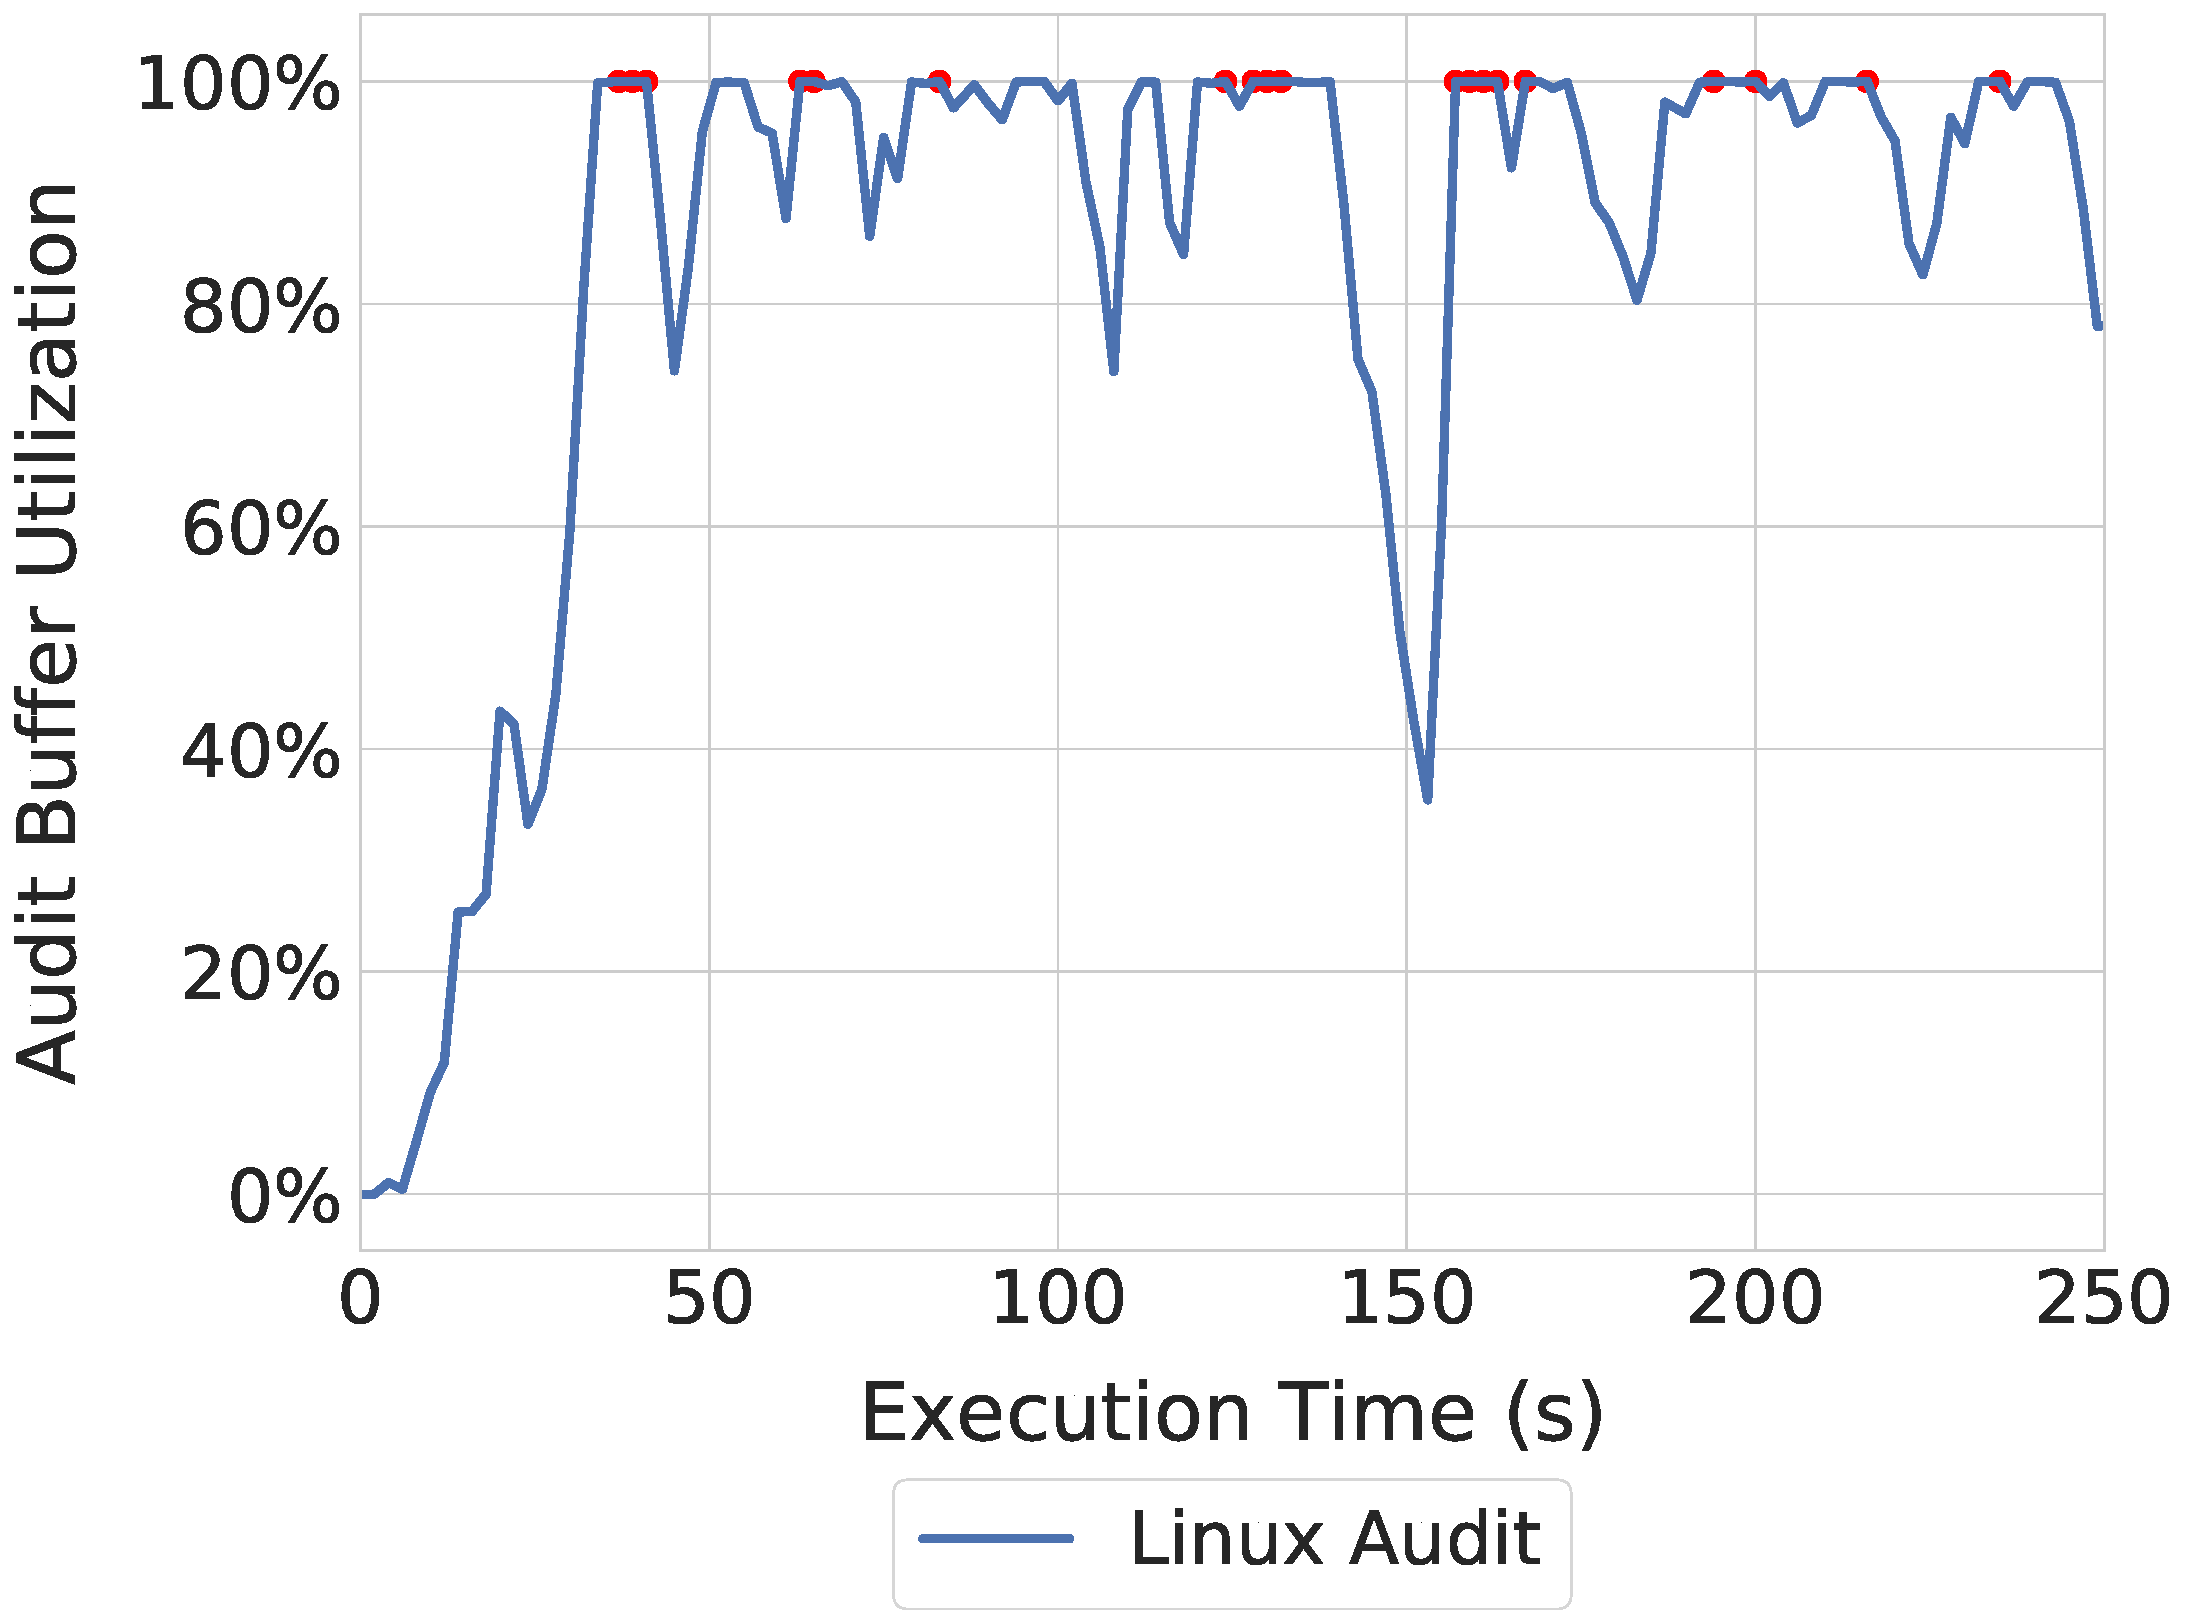
\includegraphics[width=0.9\linewidth,keepaspectratio,scale=0.9]{fig/backlog_over_time_hlight.pdf}
    \caption{\label{fig:eval_backlog}Kaudit buffer utilization over time for Linux Audit. Linux Audit's {\tt backlog} value was measured every 2 seconds during the execution of the application and plotted as a percentage of the max backlog limit.
    Additional red annotations signify all times where buffer utilization was 100\% and hence audit events might be lost. At these points Linux Audit performance is actually worse than depicted, but was constrained by the alotted buffer space.}    
\end{figure}

 For measuring the utilization of the kaudit buffer, we periodically sampled the buffer state every 2 seconds using the audit command line utility \textit{auditctl}, while executing the ArduPilot application for 100K iterations. 

\textbf{Observations:} From Figure~\ref{fig:eval_backlog}, we see that for Linux Audit, the utilization of the kaudit buffer rises quickly in the beginning and remains close to 100\% for the majority of the running time, resulting in loss of audit messages.

\textbf{Discussion:}
When the kaudit buffer is full, new audit messages are lost; hence, to ensure that suspicious events are recorded, it is essential that \textit{the buffer is never full}.
The variations that we see in the plots can be attributed to the scheduling of the non real-time \textit{kauditd} thread that is responsible for sending the outstanding audit messages to user-space for retention on disk. We observe that the backlog builds with time when \textit{kauditd} isn't scheduled and drops sharply when \textit{kauditd} eventually gets CPU time. 

As \textit{kauditd} is a non real-time thread running with no priority, it contends with multiple background processes for CPU time resulting in high buildup of messages in the kaudit buffer. Reducing the pressure of incoming audit messages using a kernel based log reduction schemef like KCAL \cite{maUsenix18} or increasing the rate of draining the kaudit buffer could be suitable approaches to ensure lossless auditing in resource constrained systems.

\subsection{Audit Latency}
\textbf{Experiment:}

\begin{figure}[tbp]
    \centering
    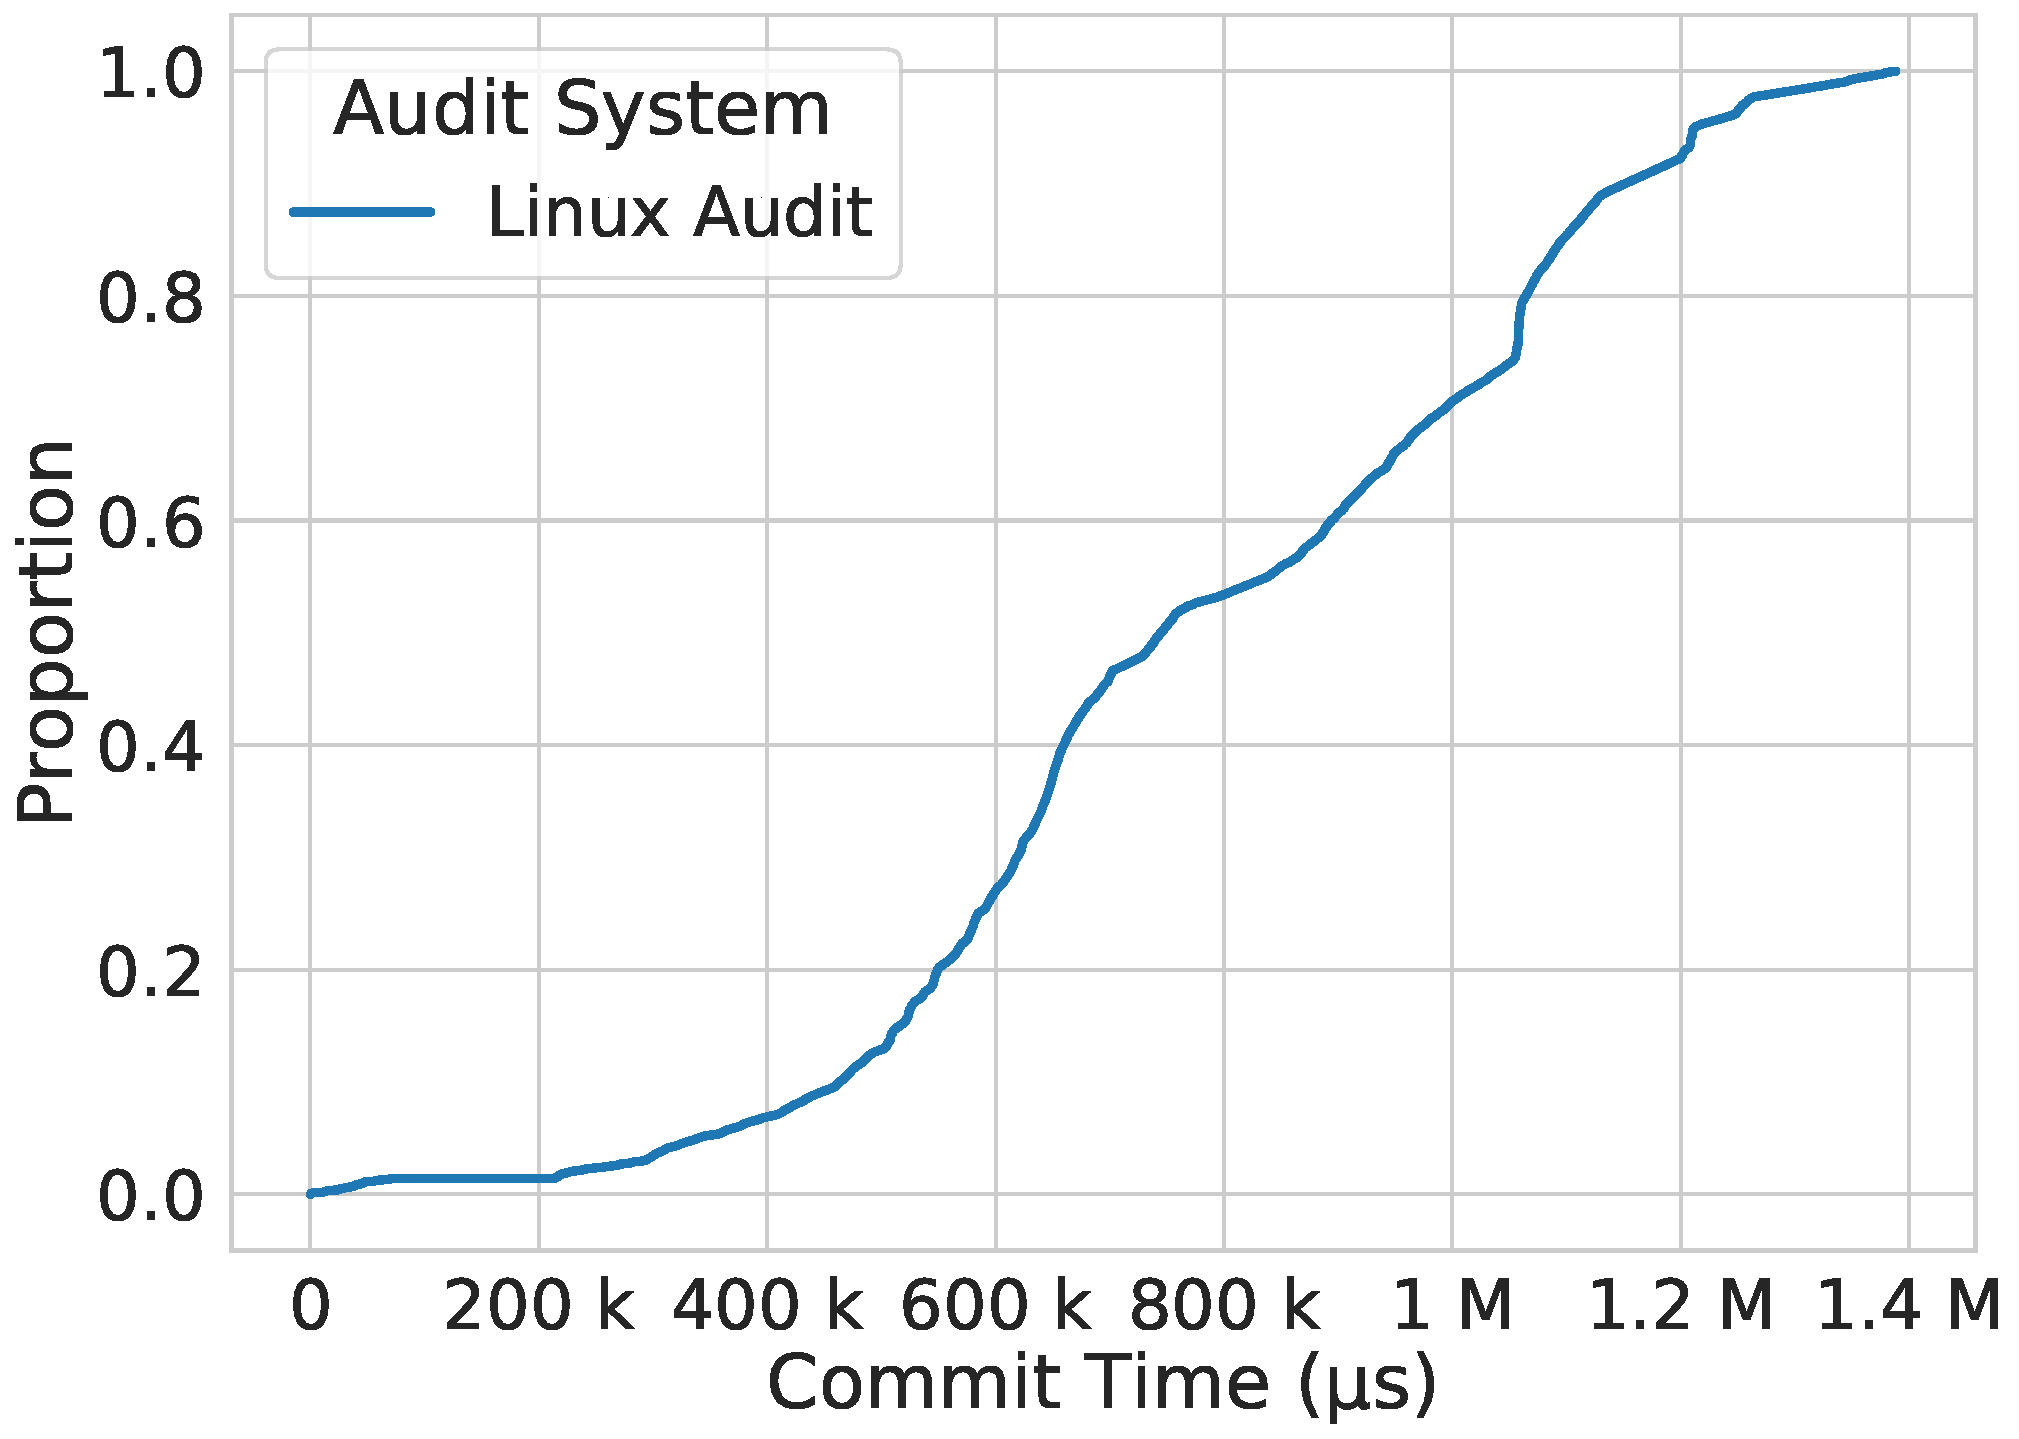
\includegraphics[width=0.9\linewidth,keepaspectratio,scale=0.9]{fig/Commit_latencies_cdf.pdf}
    \caption{\label{fig:eval_latency}Audit commit latencies over time for Linux Audit plotted as a Cumulative Distribution Function (CDF). The experiment measures the time between the generation of an audit message and before the message is written to disk in userspace by the \textit{auditd} thread. For a chosen commit time \textit{t} on the x-axis, the y-axis shows the fraction of the total messages that encountered delay of less than \textit{t} microseconds.}
\end{figure}

For measuring the amount of time each audit message spends in the audit subsystem, the ArduPilot application was executed over 10K iterations and the audit latency was computed from the commit time and the audit time of each audit message obtained from the log file. The non real time \textit{kauditd} and \textit{auditd} threads are run with a nice value of 0 and -4 respectively.

\textbf{Observations:} From Figure~\ref{fig:eval_latency}, we see that the audit latencies across 140k audit messages has a very wide range from 130 microseconds to 1.38 seconds with a median of \~740 ms. 

\textbf{Discussion:} 
The wide range of audit latencies points us to the fact that vanilla Linux Audit maybe a poor choice for real time systems, which typically demand predictable and tightly bound temporal performance guarantees. The low observed minimum audit latency suggests that the implementation of the audit subsystem itself may not entirely to blame for the high \textit{kauditd} buffer utilization and reinforces our earlier observation that scheduling of audit threads is the primary reason for the long tail in audit latencies.

As the audit threads execute at lower non real time priorities, they rely on adequate application slack time to complete execution. With the introduction of synchronous and asynchronous overheads of auditing, the effective slack time reduces further taking away CPU time from the audit subsystem. Reliably accounting for these auditing overheads and increasing priorities of audit threads could help design a schedulable audited RT system and reign in the tail audit latencies.

\subsection{Audit Throughput}
\textbf{Experiment:}
\begin{figure}[tbp]
    \centering
    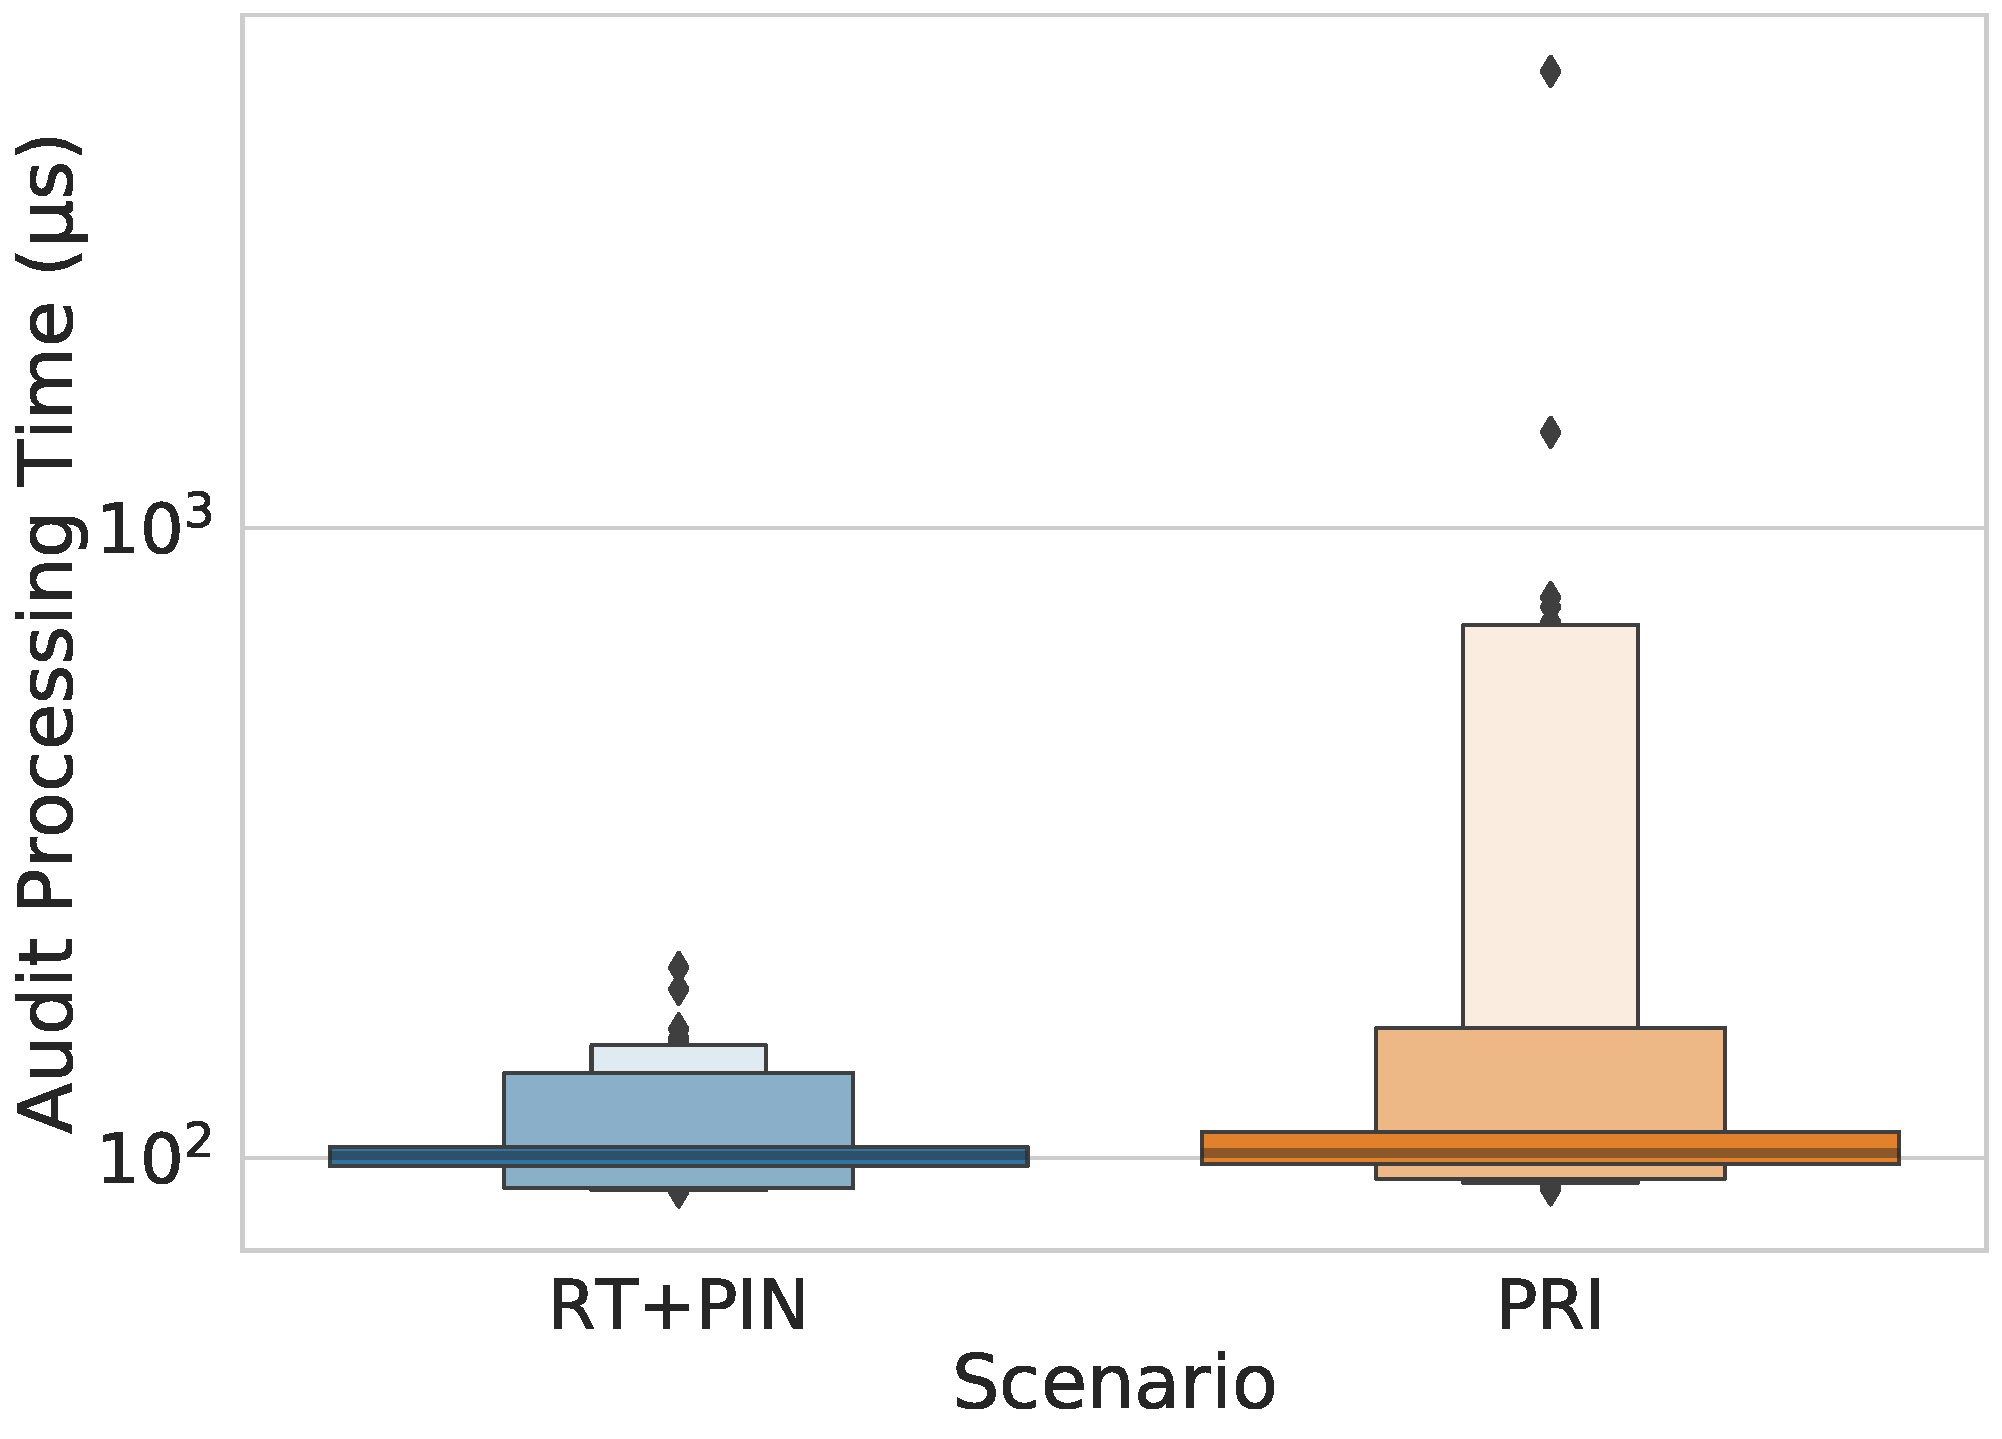
\includegraphics[width=0.9\linewidth,keepaspectratio,scale=0.9]{fig/Throughput_cdf.pdf}
    \caption{\label{fig:eval_throughput}Audit Processing Time .}
\end{figure}

For measuring the amount of time required to process a single audit message by the audit subsystem only, we ran a microbenchmark application that consisted of 10 \textit{getpid} system calls and observed the intervals at which audit messages were written to disk over 10 runs. In the RT+PIN scenario, both audit threads were assigned a low real time priority and the \textit{auditd} thread was pinned to core 2 on the machine. As \textit{kauditd} is a kernel thread, we weren't able to pin the thread to a fixed core on the system, instead relying on its real time priority to ensure that it ran ahead of any background process. Whereas in the PRI scenario, the priorities of the audit threads were increased by modifying their nice values, which resembles the default configuration of the audit subsystem.

\textbf{Observations:} From Figure~\ref{fig:eval_throughput}, we observe that for the PRI case, the interval for processing audit messages varies from 88 $\mu$s to 5ms. Introducing real time priorities and core pinning reduces the variance in measurements and reduces the maximum interval to 200 $\mu$s.

\textbf{Discussion:} \todo[inline]{Wrap up discussion - fairly obvious that low priority + core pinning would have worked - reduces time wasted in moving task around and moves it above background task, ensures CPU time -  need to add an additional core to ensure enough CPU time for the buffer - that could be reasonable as it can be factored in during the design phase itself - having an upper bound on the audit throughput helps plan for schedulability}

\subsection{Summary of Results}
\todo[inline]{Summarize takeaways - timing comes in handy to understand resource allocation - we can understand if log reduction is required once we are maxed out on our resource allocation.}